\section{Фазовые решетки}


% \red{Эффект мультипицирования, принципы пространственной фильтрации}


% \begin{to_def}
%     Объект называется \textit{абсорбционным}, если в различных местах обладает различной прозрачностью. Объект называется \textit{рефракционным}, если не поглощает света, но влиеяет на фазу. 
% \end{to_def}



% \subsection{Применение метода Рэлея}


\textbf{Амплитудная решетка}. Есть решетка с щелями ширины $b$ и непрозрачных промежутков между ними ширины $a$. Начало координат в середине щели:
\begin{equation*}
    D_m = \frac{1}{d} \int_{-d/2}^{+d/2} D(x) e^{impx} \d x = 
    \frac{1}{d} \int_{-b/2}^{+b/2} e^{impx} \d x = \frac{b}{d} \frac{\sin \varkappa}{\varkappa},
    \hspace{5 mm}  
    \varkappa = \pi \frac{m b}{d}.
\end{equation*}
Что верно при малых углах дифракции, с $\cos \theta \approx 1$. Для спектра нулевого порядка $D_0 = b/d$, и $I_0 = (b/d)^2$, а полна $\sub{I}{прош} = b/d$, вообще верно, что
\begin{equation*}
    \frac{b}{d} = \frac{b^2}{d^2} + \frac{2}{\pi^2} \sum_{m=1}^{\infty} \frac{1}{m^2} \sin^2 \frac{\pi m b}{d}.
\end{equation*}
Относительная доля дифрагированного света
\begin{equation*}
    \frac{\sub{I}{прош} - I_0}{\sub{I}{прош}} = 1 - \frac{b}{d}.
\end{equation*}
Стоит помнить, что $d \sin \vartheta = m \lambda$. 





\textbf{Амплитудно-фазовая решётка.} Пусть есть участки длины $b$ с пропускаемостью $\beta$ и участки длины $a$ с пропускаемостью $\alpha$, где $\alpha$ и $\beta$ постоянны. 

Вычисение $D_m$ сводится к предыдущей задаче. Рассматриваемая решётка эквивалентна плоскопараллеьной решетке с пропусканием $\alpha$ и наложенной на неё дифракционной решетки пропускаемости $(\beta-\alpha)$. Так приходим к выражению
\begin{equation*}
    D_m = (\beta-\alpha) \frac{b}{d} \frac{\sin(\varkappa)}{\varkappa} + \alpha \delta_m, \hspace{5 mm} 
    \varkappa = \pi \frac{ m b}{d},
\end{equation*}
где $\delta_m = 1$ при $m=0$ и $\delta_m = 0$ при $m \neq 0$. В случае фазовой реешетки пропускаемости имеют вид $e^{i \rho}$, так как важна лишь разность фаз, то вполне можем положить $\alpha=1$ и $\beta=e^{i \rho}$. Тогда
\begin{align*}
    D_m &= (e^{i \rho}-1) \frac{b}{d} \frac{\sin\varkappa}{\varkappa}, \hspace{5 mm} m \neq 0, \\
    D_0 &= (e^{i \rho} -1) \frac{b}{d} + 1.
\end{align*}
Итого имеет дополнительный сдвиг фаз между спектром нулевого и спектрами всех прочих порядков. Можем его найти, посчитав
\begin{equation*}
    \arg \frac{D_m}{D_0} = \varphi, \hspace{5 mm} \tg \varphi = \frac{b+a}{b-a} \frac{\sin \rho}{1-\cos \rho}.
\end{equation*}
Введя на пути нулевого максимума пластину, меняющую фазу на $\varphi$ можем перейти к фазовым соотношениями, аналогичным амплитудной решетке, на основе этого и строится \textit{метод фазового контраста}. 

Стоит заметить, что при $a=b$ $\varphi =\pi/2$, а при $\rho \ll 1$  получим $\varphi \approx \pi/2$. 


\textbf{Эшелетт}. \red{Сивухин, страница 362.}



% 

% см. 53
% 400






\textbf{Идея фазового контраста}. Пусть два разных участка формируют векторы $\vc{A}$ и $\vc{B}$, при чём после фазовое решетки $|\vc{A}|$ близок к $|\vc{B}|$, но повернуты на некоторый угол (рис. \ref{fig:pfc59}, а).
\begin{figure}[ht]
    \centering
    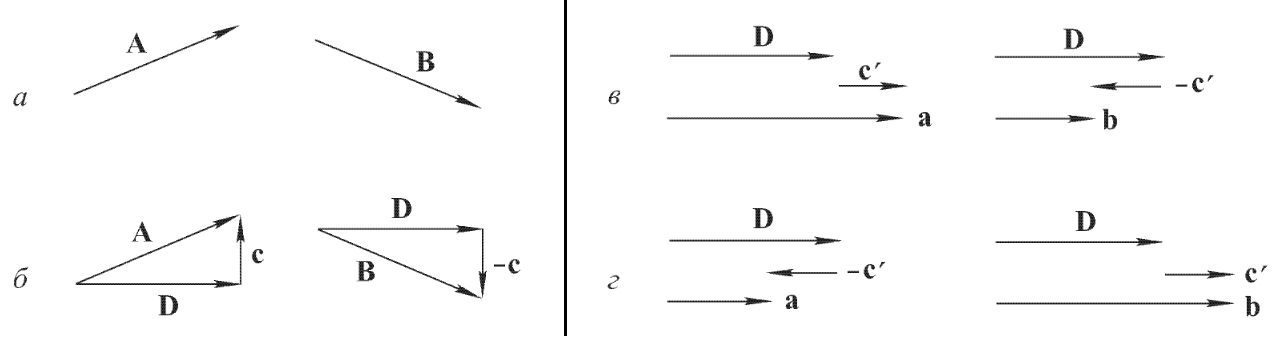
\includegraphics[width=0.65\textwidth]{figures/59_1.png}
    \caption{Метод фазового контраста}
    \label{fig:pfc59}
\end{figure}
Если повернуть $\vc{c}'$ и $\vc{c}$ на $\pi/2$, оставляя неизменным $\vc{D}$, то можем получить \textit{позитивный фазовый контраст} (в) и негативный фазовый контраст (г). 



\textbf{Реализация}. Прежде всего необходимо пространственно разделить волновые поля, представленные веткорами $\vc{c}$ и $\vc{D}$. Полное колебание имеет постоянную амплитуду на протяжении всей реешетки  и изображается вектором $\vc{D}$, оно даёт в фокальной плоскости центральный максимум, и только. 

Другое колебание представляется периодической функцией принимающую значения от $-\vc{c}$ до $\vc{c}$ на соседних участках, в среднем ноль, так что возбуждает только боковые максимумы, таким образом в фокальной плоскости объектива оба колебания окажутся пространственно разделенными. 

Поставив на пути либо центрального максимума, либо всех боковых максимумов прозрачную плоскопараллельную фазовую пластинке нужной тощины, можно ввести разность фаз в $\pi/2$ и так осуществить фазовый контраст. 


Стоит заметить, что раньше полная энергия на участках решётки была $2(D^2 + c^2)$, а после повтора $\vc{c}$ и $-\vc{c}$ энергия становится $(D+c)^2 + (D-c)^2$, то есть сохранятся, но перераспределяется. 








\red{Дописать 
9.15,
9.22,
9.17,
9.19,
метод темного поля,
метод фазового контраста, метод дефокусировки, 
}
